  \begin{tikzpicture}
    \tikzset{v composant/.style={visible on=<1-2>},
      vv systeme/.style={visible on=<2>},
      v systeme/.style={visible on=<2->},
      v comparaison/.style={visible on=<3->},
%
      equation composant/.style={cellule, align=center, anchor=north, font=\small,
        fill=white, v composant},
%
      carac etiquette/.style={etiquette, below=1.5em, v comparaison},
      carac composant/.style={align=left, , v comparaison, font cellule},
      carac systeme/.style={align=left, v comparaison, font cellule},
};


\node[cellule] (systeme) at (0,0) {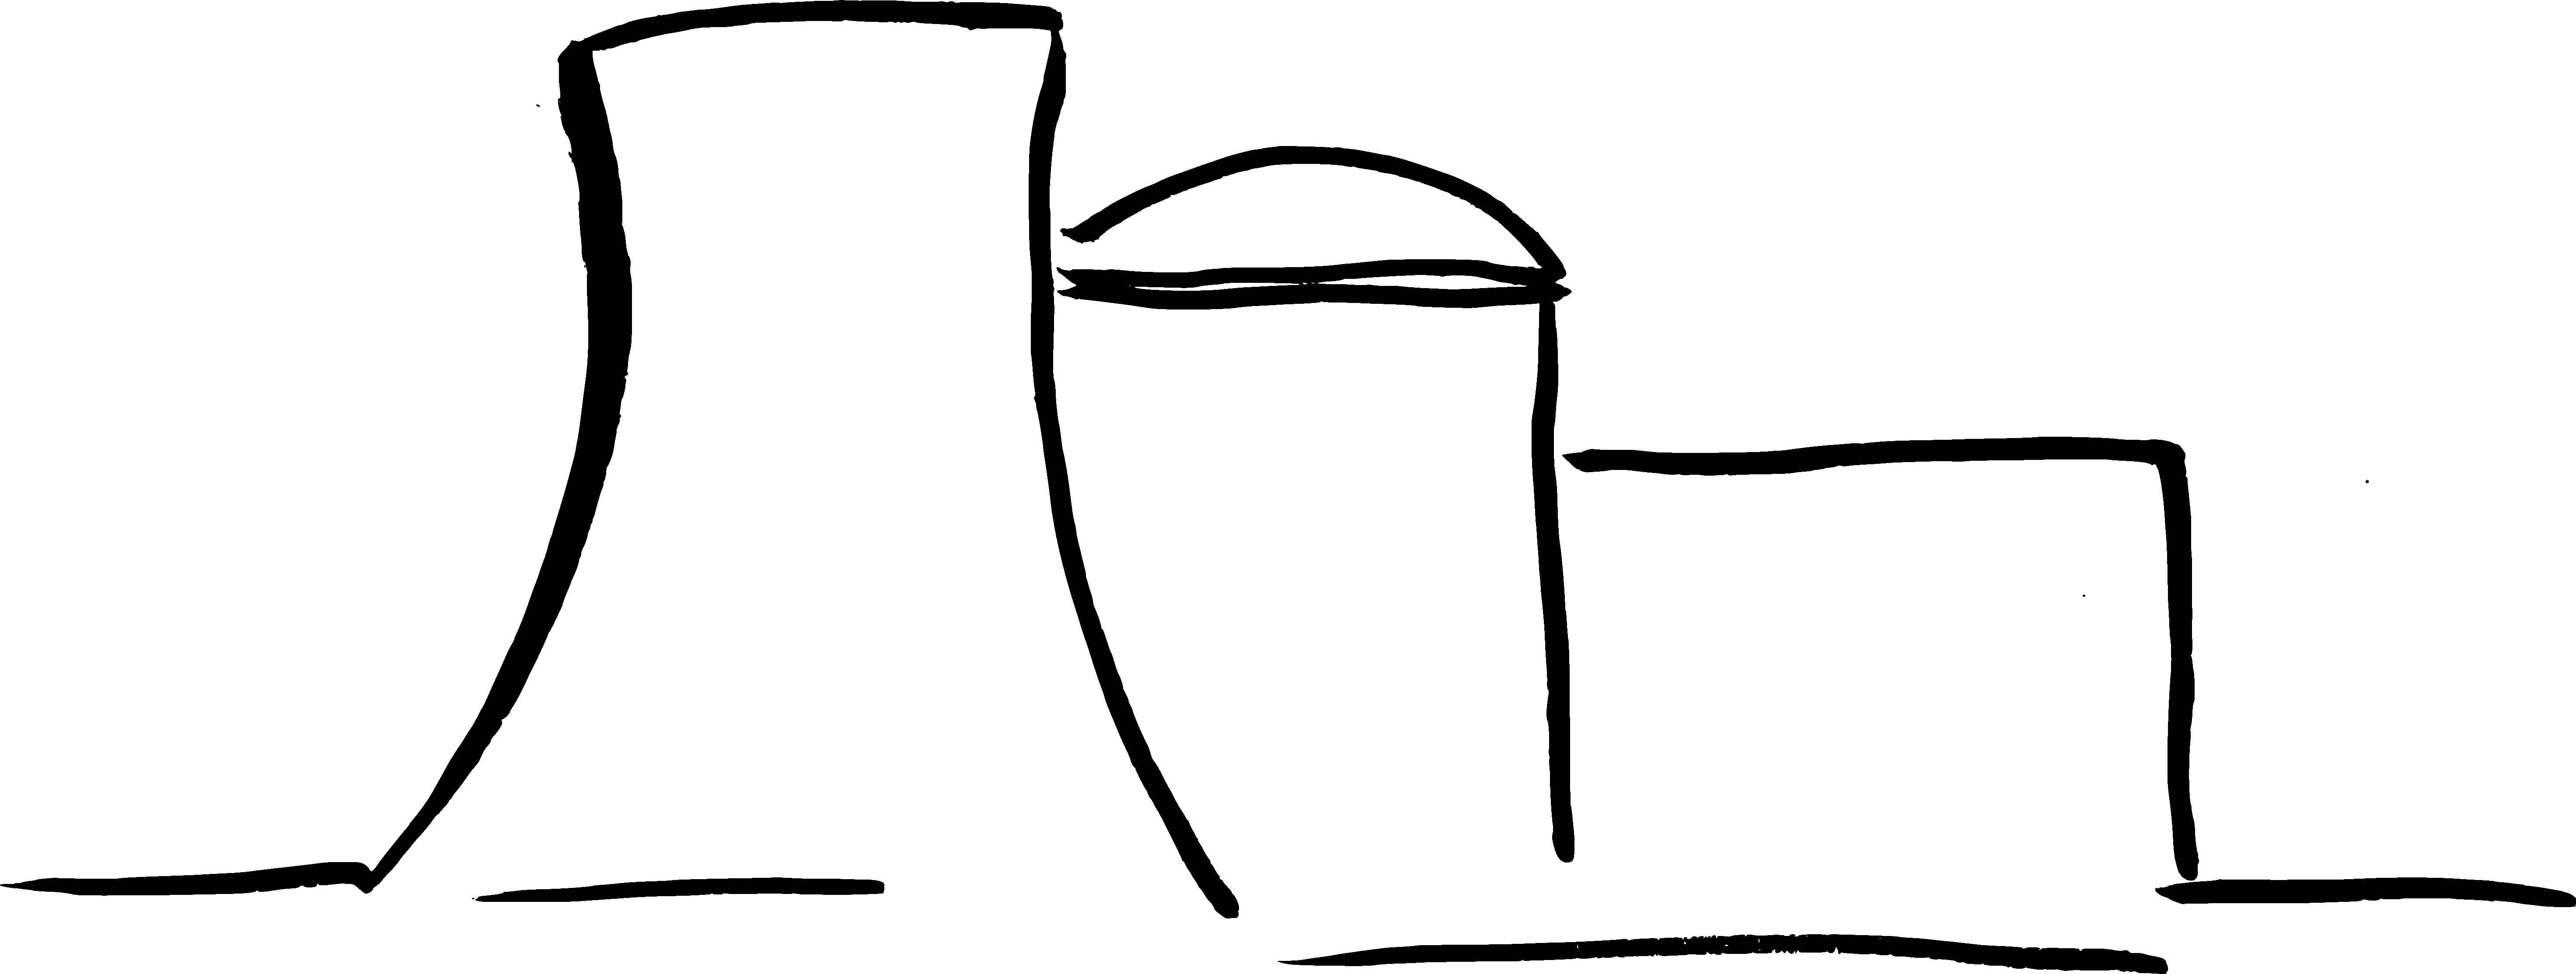
\includegraphics[height=1.3cm]{./figure/npp}};

\node[cellule, below right=3mm and 5mm, vv systeme] (decoupage) at (systeme.south east) {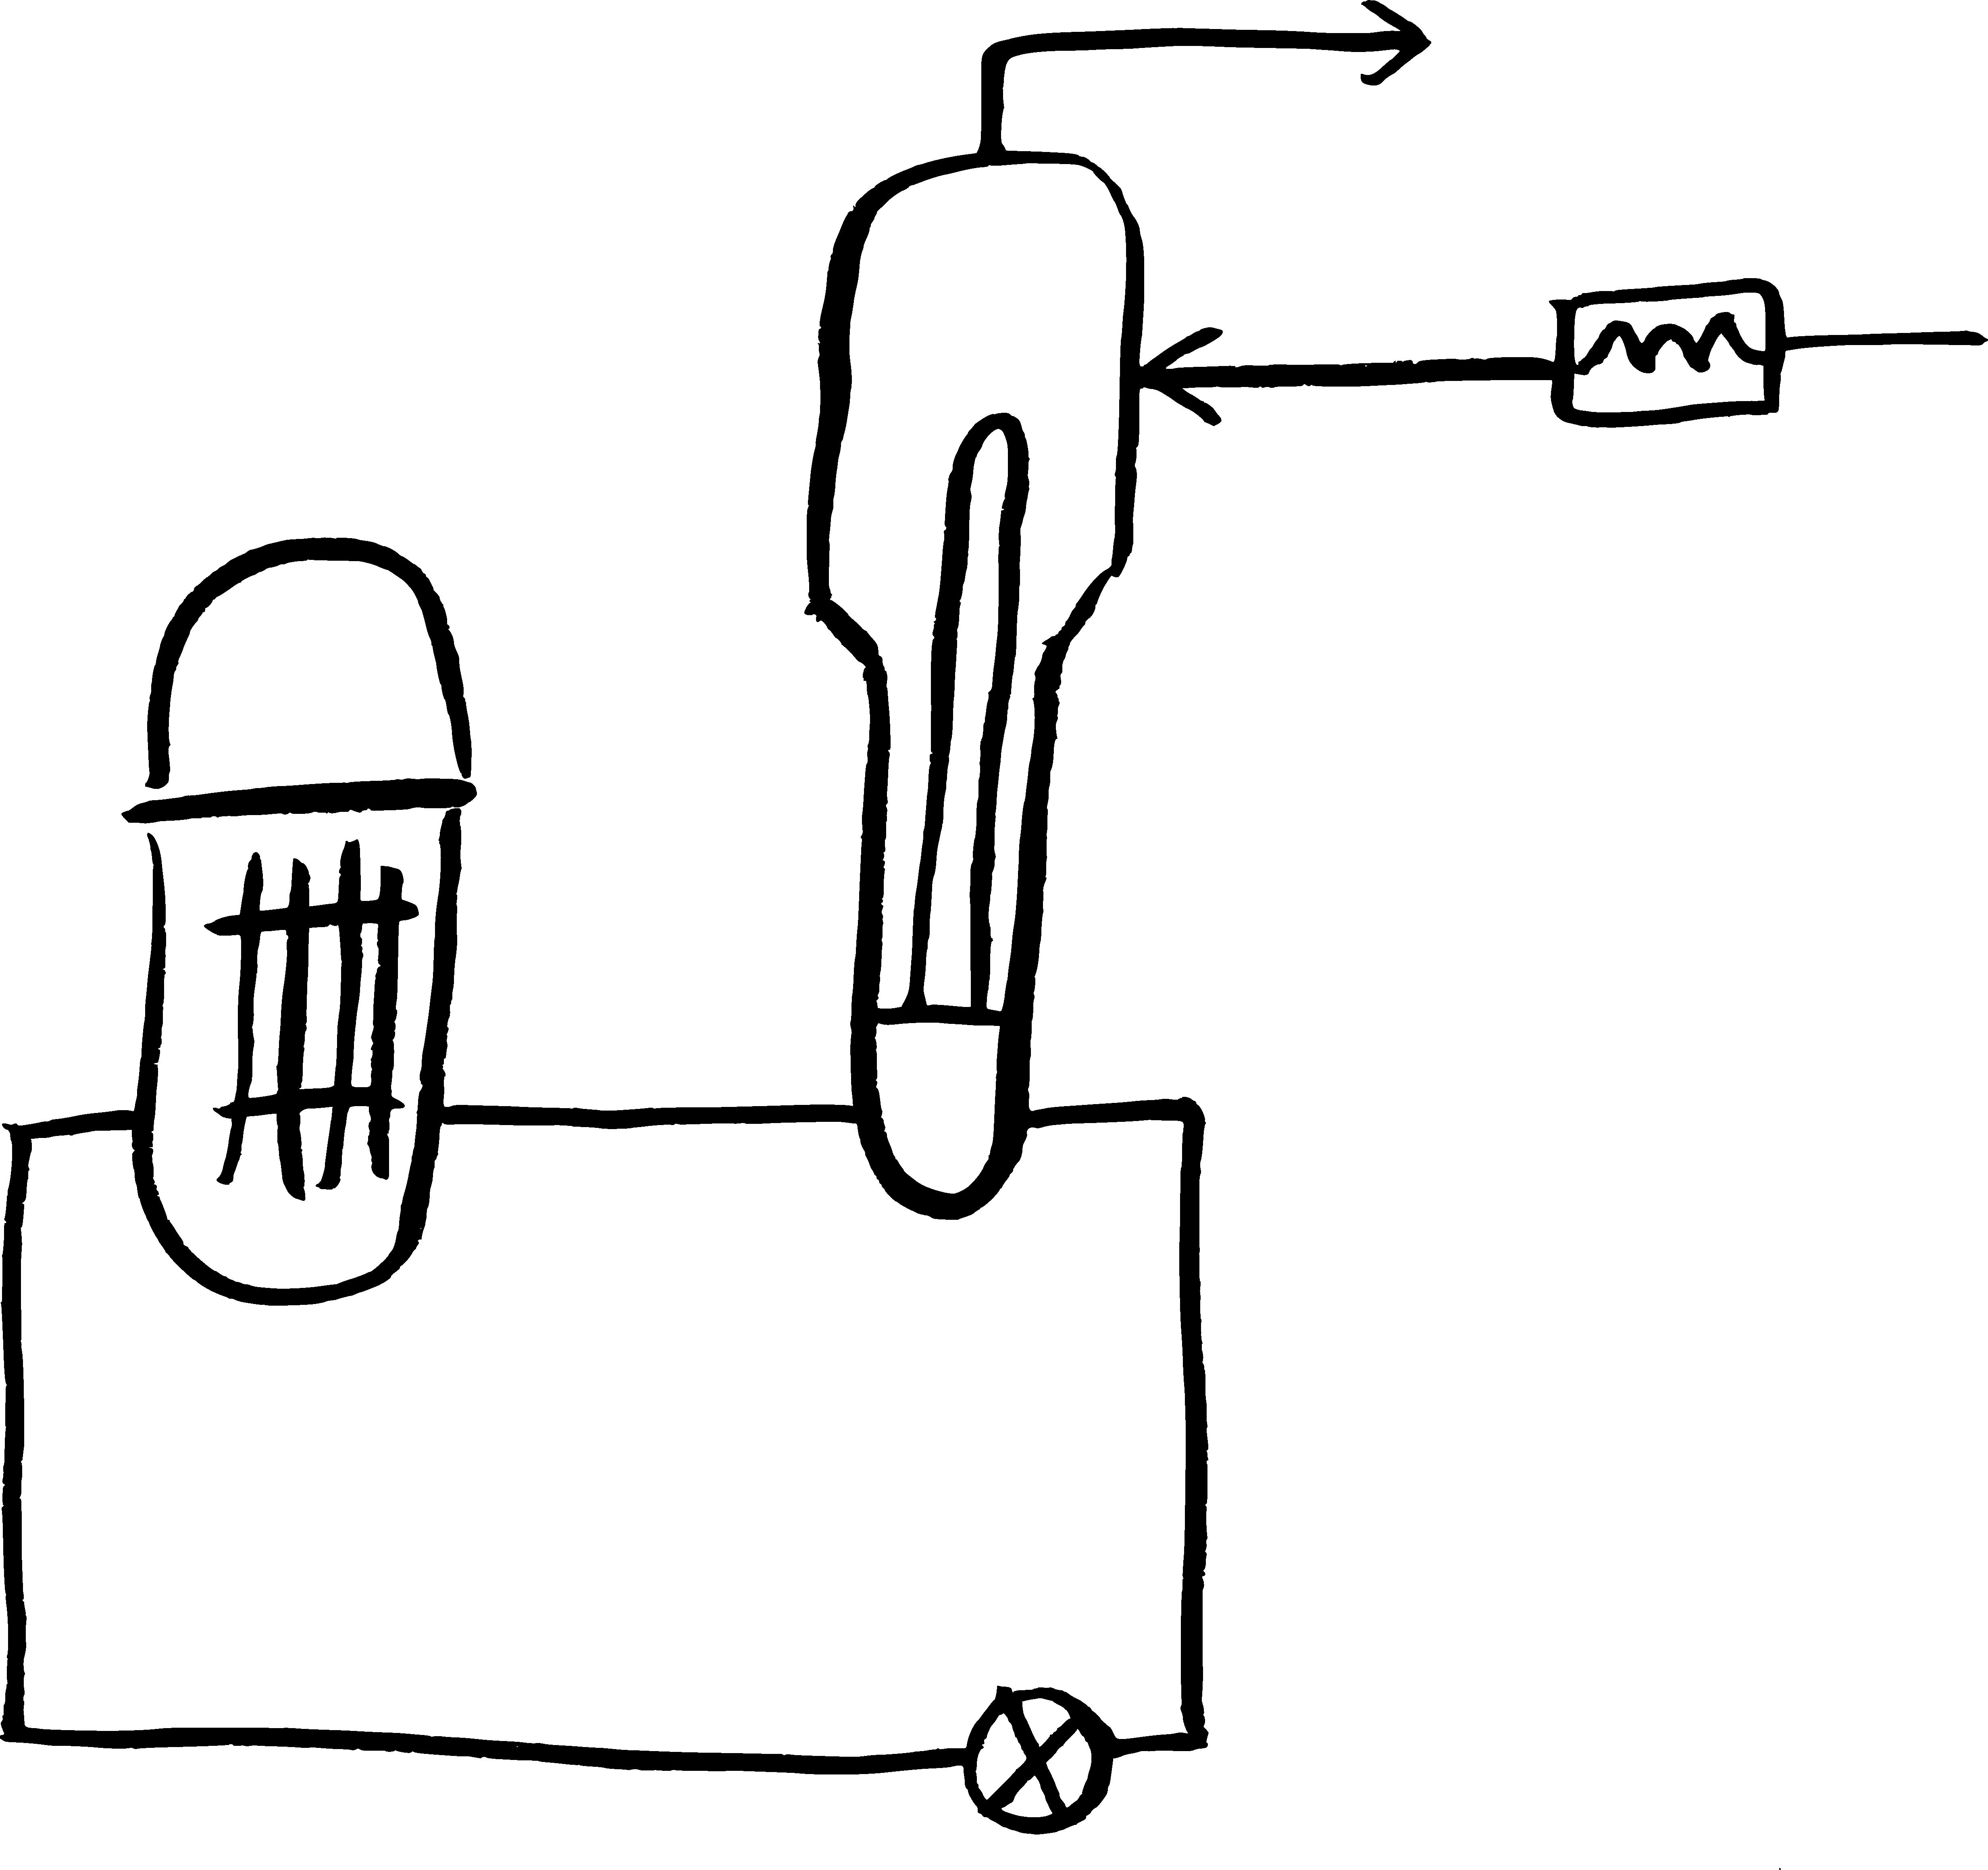
\includegraphics[height=2.2cm]{./figure/decoupage_c}};


\node[cellule, v composant, below left=3mm and 5mm] (gv) at (systeme.south west) {
\includegraphics[height=2.2cm]{./figure/gv}};
\node[cellule, v composant, left=1mm] (cuve) at (gv.west) {
\includegraphics[height=2.2cm]{./figure/cuve}};
\node[cellule, v composant, left=1mm] (pompe) at (cuve.west) {
\includegraphics[height=.5cm]{./figure/pompe}};

\node[cellule, below=3mm, align=center, font=\small, vv systeme] (equation) at (decoupage.south) {\systemeequation};

\node[equation composant, xshift=13mm] (equation pompe) at (pompe.south |- equation.north) {\systemeequation};
\node[equation composant, right=2mm] (equation cuve) at (equation pompe.west) {\systemeequation};
\node[equation composant, right=2mm] (equation gv) at (equation cuve.west) {\systemeequation};

\coordinate[yshift=-12mm] (code) at (equation.south);
\pic[file style, "Modelica", vv systeme, xshift=12mm]  at (code) {file icon};
\pic[file style, "Symulink", vv systeme, xshift=-12mm]  at (code) {file icon};

\pic[file style, "C++", v composant] at (pompe |- code) {file icon};
\pic[file style, "Éléments finis", xshift=4mm, v composant] at (cuve |- code) {file icon};
\pic[file style, "CFD", xshift=6mm, v composant] at (gv |- code) {file icon};


\node[etiquette, above=1mm, xshift=-2mm] at (systeme.east) {Real system};

\node[etiquette, v composant] (etiquette decoupage) at (systeme |- decoupage) {“Packing”};
\node[etiquette, v composant] (etiquette equation) at (systeme |- equation) {Equation formulation};
\node[etiquette, v composant, align=center] at (systeme |- code) {Solver\\programming};

% En-tête
\node[cellule,  align=center, draw=none, v systeme] (titre systeme) at (systeme -| decoupage) {0D/1D\\system modelling};
\node[cellule, align=center, draw=none] (titre composant) at (systeme -| cuve) {“Regular”\\modelling};

% Séparation réel-modèle
\draw[thick, dashed, gray] ([yshift=-1.5mm]systeme.south west -| equation pompe.west)--([yshift=-1.5mm]systeme.south west -| equation.east);

% ================
\coordinate (tmp) at (systeme.south);

\node[carac etiquette] (tmp) at (tmp.south) {CPU time};
\node[carac composant] at (tmp -| titre composant) {Long (minute $\rightarrow$ hour)};
\node[carac systeme] at (tmp -| titre systeme) {Short (second $\rightarrow$ minute)};



\node[carac etiquette] (tmp) at (tmp.south) {Dimensions};
\node[carac composant] at (tmp -| titre composant) {2D, 3D};
\node[carac systeme] at (tmp -| titre systeme) {0D, 1D};

\node[carac etiquette] (tmp) at (tmp.south) {Development rate};
\node[carac composant] at (tmp -| titre composant) {Discrete versioning};
\node[carac systeme] at (tmp -| titre systeme) {Continuous mutation};

\node[carac etiquette] (tmp) at (tmp.south) {Actors};
\node[carac composant] at (tmp -| titre composant) {Numerical analyst, physicist};
\node[carac systeme] at (tmp -| titre systeme) {Design, process, operation\ldots\\engineer};

% \node[carac etiquette] (tmp) at (tmp.south) {Équations de fermeture};
% \node[carac composant] at (tmp -| titre composant) {Phénoménologiques};
% \node[carac systeme] at (tmp -| titre systeme) {Empiriques};


\node[carac etiquette] (tmp) at (tmp.south) {Tools};
\node[carac composant] at (tmp -| titre composant) {CFD, finite elements,\\C++, FORTRAN\ldots};
\node[carac systeme] at (tmp -| titre systeme) {Modelica, Simulink\ldots};

  \end{tikzpicture}
